\documentclass[journal,12pt,twocolumn]{IEEEtran}

\usepackage{setspace}
\usepackage{gensymb}
\singlespacing
\usepackage[cmex10]{amsmath}

\usepackage{amsthm}

\usepackage{mathrsfs}
\usepackage{txfonts}
\usepackage{stfloats}
\usepackage{bm}
\usepackage{cite}
\usepackage{cases}
\usepackage{subfig}

\usepackage{float}

\usepackage{longtable}
\usepackage{multirow}

\usepackage{enumitem}
\usepackage{mathtools}
\usepackage{steinmetz}
\usepackage{tikz}
\usepackage{circuitikz}
\usepackage{verbatim}
\usepackage{tfrupee}
\usepackage[breaklinks=true]{hyperref}
\usepackage{graphicx}
\usepackage{tkz-euclide}

\usetikzlibrary{calc,math}
\usepackage{listings}
    \usepackage{color}                                            %%
    \usepackage{array}                                            %%
    \usepackage{longtable}                                        %%
    \usepackage{calc}                                             %%
    \usepackage{multirow}                                         %%
    \usepackage{hhline}                                           %%
    \usepackage{ifthen}                                           %%
    \usepackage{lscape}     
\usepackage{multicol}
\usepackage{chngcntr}

\DeclareMathOperator*{\Res}{Res}

\renewcommand\thesection{\arabic{section}}
\renewcommand\thesubsection{\thesection.\arabic{subsection}}
\renewcommand\thesubsubsection{\thesubsection.\arabic{subsubsection}}

\renewcommand\thesectiondis{\arabic{section}}
\renewcommand\thesubsectiondis{\thesectiondis.\arabic{subsection}}
\renewcommand\thesubsubsectiondis{\thesubsectiondis.\arabic{subsubsection}}


\hyphenation{op-tical net-works semi-conduc-tor}
\def\inputGnumericTable{}                                 %%

\lstset{
%language=C,
frame=single, 
breaklines=true,
columns=fullflexible
}
\begin{document}

\newcommand{\BEQA}{\begin{eqnarray}}
\newcommand{\EEQA}{\end{eqnarray}}
\newcommand{\define}{\stackrel{\triangle}{=}}
\bibliographystyle{IEEEtran}
\raggedbottom
\setlength{\parindent}{0pt}
\providecommand{\mbf}{\mathbf}
\providecommand{\pr}[1]{\ensuremath{\Pr\left(#1\right)}}
\providecommand{\qfunc}[1]{\ensuremath{Q\left(#1\right)}}
\providecommand{\sbrak}[1]{\ensuremath{{}\left[#1\right]}}
\providecommand{\lsbrak}[1]{\ensuremath{{}\left[#1\right.}}
\providecommand{\rsbrak}[1]{\ensuremath{{}\left.#1\right]}}
\providecommand{\brak}[1]{\ensuremath{\left(#1\right)}}
\providecommand{\lbrak}[1]{\ensuremath{\left(#1\right.}}
\providecommand{\rbrak}[1]{\ensuremath{\left.#1\right)}}
\providecommand{\cbrak}[1]{\ensuremath{\left\{#1\right\}}}
\providecommand{\lcbrak}[1]{\ensuremath{\left\{#1\right.}}
\providecommand{\rcbrak}[1]{\ensuremath{\left.#1\right\}}}
\theoremstyle{remark}
\newtheorem{rem}{Remark}
\newcommand{\sgn}{\mathop{\mathrm{sgn}}}
\providecommand{\abs}[1]{\vert#1\vert}
\providecommand{\res}[1]{\Res\displaylimits_{#1}} 
\providecommand{\norm}[1]{\lVert#1\rVert}
%\providecommand{\norm}[1]{\lVert#1\rVert}
\providecommand{\mtx}[1]{\mathbf{#1}}
\providecommand{\mean}[1]{E[ #1 ]}
\providecommand{\fourier}{\overset{\mathcal{F}}{ \rightleftharpoons}}
%\providecommand{\hilbert}{\overset{\mathcal{H}}{ \rightleftharpoons}}
\providecommand{\system}{\overset{\mathcal{H}}{ \longleftrightarrow}}
	%\newcommand{\solution}[2]{\textbf{Solution:}{#1}}
\newcommand{\solution}{\noindent \textbf{Solution: }}
\newcommand{\cosec}{\,\text{cosec}\,}
\providecommand{\dec}[2]{\ensuremath{\overset{#1}{\underset{#2}{\gtrless}}}}
\newcommand{\myvec}[1]{\ensuremath{\begin{pmatrix}#1\end{pmatrix}}}
\newcommand{\mydet}[1]{\ensuremath{\begin{vmatrix}#1\end{vmatrix}}}
\numberwithin{equation}{subsection}
\makeatletter
\@addtoreset{figure}{problem}
\makeatother
\let\StandardTheFigure\thefigure
\let\vec\mathbf
\renewcommand{\thefigure}{\theproblem}
\def\putbox#1#2#3{\makebox[0in][l]{\makebox[#1][l]{}\raisebox{\baselineskip}[0in][0in]{\raisebox{#2}[0in][0in]{#3}}}}
     \def\rightbox#1{\makebox[0in][r]{#1}}
     \def\centbox#1{\makebox[0in]{#1}}
     \def\topbox#1{\raisebox{-\baselineskip}[0in][0in]{#1}}
     \def\midbox#1{\raisebox{-0.5\baselineskip}[0in][0in]{#1}}
\vspace{3cm}
\title{\textbf{Gate Assignment 1}}
\author{Vijay Varma - AI20BTECH11012}
\maketitle
\newpage
\bigskip
\renewcommand{\thefigure}{\theenumi}
\renewcommand{\thetable}{\theenumi}
%
Download latex-tikz codes from 
%
\begin{lstlisting}
https://github.com/KBVijayVarma/EE3900/tree/main/Gate_Assignment_1
\end{lstlisting}
Download python codes from 
%
\begin{lstlisting}
https://github.com/KBVijayVarma/EE3900/tree/main/Gate_Assignment_1/code
\end{lstlisting}

\section*{\textbf{Problem (Vectors Q2.14)}}
Two systems with impulse responses $h_1$(t) and $h_2$(t) are connected in cascade. Then the overall 
impulse response of the cascaded system is given by
\begin{enumerate}
   \item product of $h_1$(t) and $h_2$(t)
   \item sum of $h_1$(t) and $h_2$(t) 
   \item convolution of $h_1$(t) and $h_2$(t) 
   \item subtraction of $h_2$(t) from $h_1$(t) 
\end{enumerate}
\section*{\textbf{Solution}}

Given Two systems with impulse responses $h_1$(t) and $h_2$(t) are connected in cascade.

We know that "when two systems are cascaded, then the resultant response is the convolution of the individual responses".

Let Input x for Cascaded System be as in the below figure. \\

\begin{figure}[!ht]
    \centering
    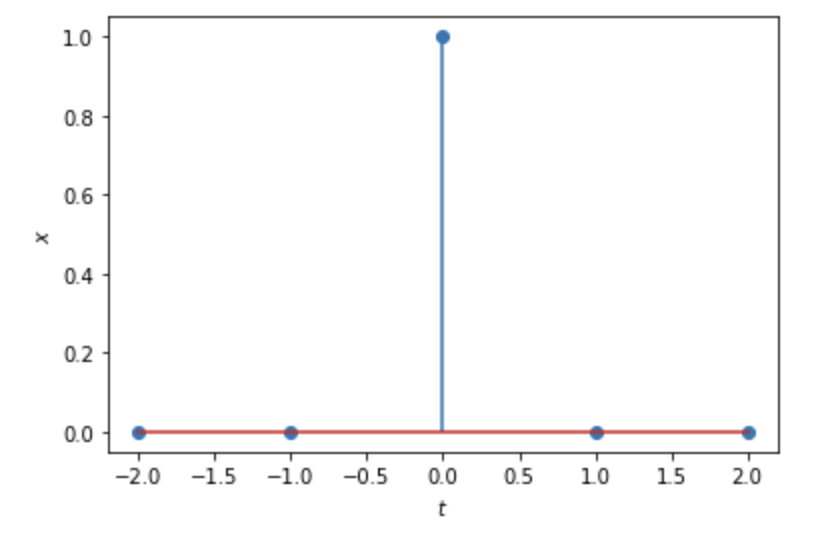
\includegraphics[width=\columnwidth]{fig1.png}
    \caption{Plot of $x$}
    \label{x}
\end{figure}

$h_1[t]$ is given by,

\begin{figure}[H]
    \centering
    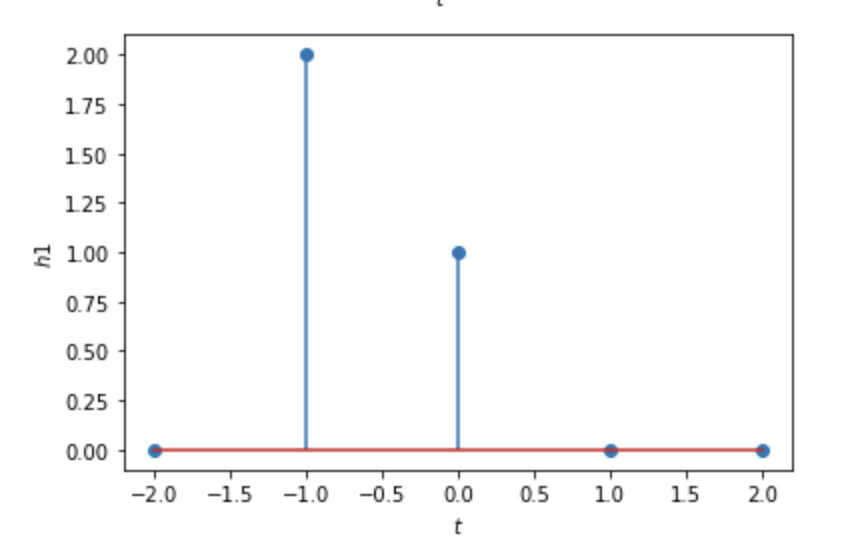
\includegraphics[width=\columnwidth]{fig2.png}
    \caption{Plot of $h1$}
    \label{h1}
\end{figure}

$h_22[t]$ is given by,

\begin{figure}[!h]
    \centering
    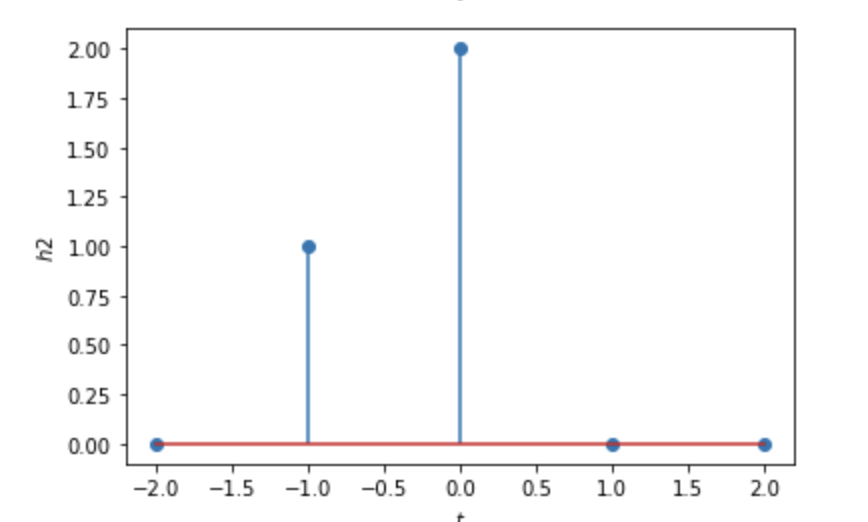
\includegraphics[width=\columnwidth]{fig3.png}
    \caption{Plot of $h2$}
    \label{h2}
\end{figure}

Now, for the cascaded system, 
\begin{align}
    y_1[t] &= x[t] * h_1[t] \\
    y_2[t] &= y_1[t] * h_2[t]
\end{align}

The final output $y_2[t]$ is given by,

\begin{figure}[H]
    \centering
    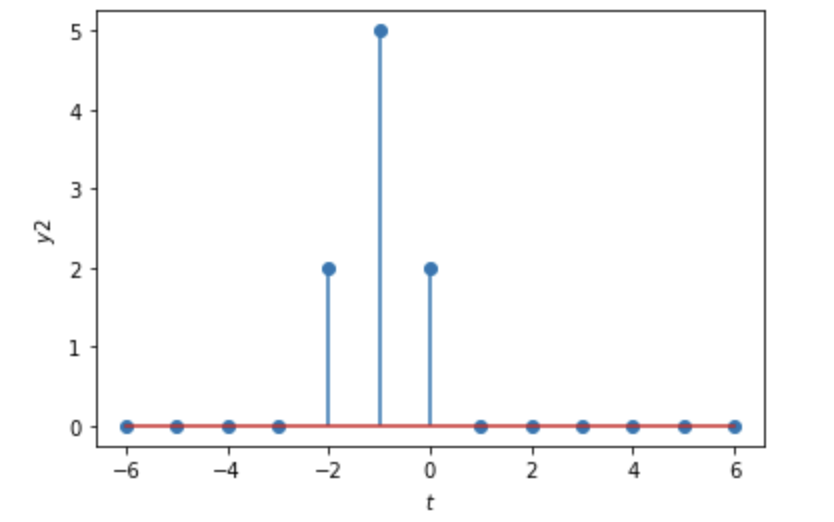
\includegraphics[width=\columnwidth]{fig4.png}
    \caption{Plot of $y2$}
    \label{y2}
\end{figure}

Now, by replacing the above method with Convolution of $h_1[t]$ and $h_2[t]$,

\begin{align}
    h[t] &= h_1[t] * h_2[t] \\
    y[t] &= x[t] * h[t]
\end{align}

In this case, the final output $y[t]$ is given by,

\begin{figure}[!h]
    \centering
    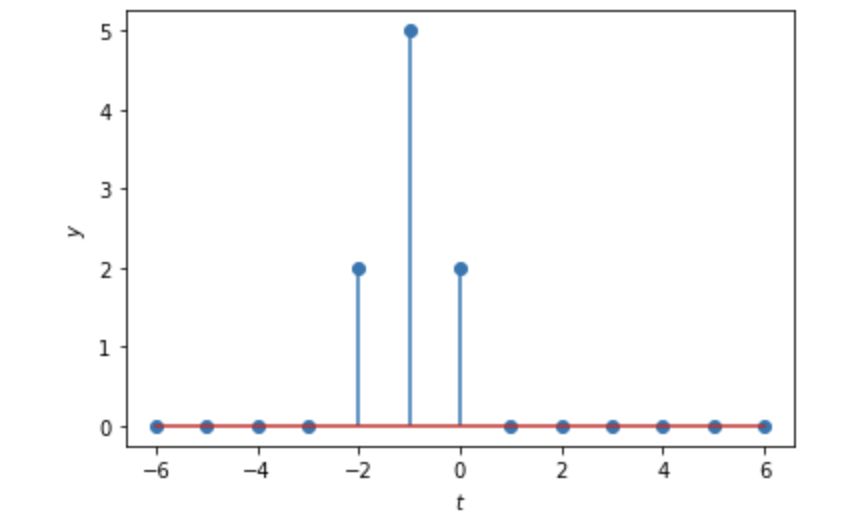
\includegraphics[width=\columnwidth]{fig5.png}
    \caption{Plot of $y$}
    \label{y}
\end{figure}

Hence, from the figures \ref{y2}, \ref{y}, the final output is the same.

Hence, the overall impulse response of the Cascaded system is given by \textbf{Convolution of $h_1$(t) and $h_2$(t)}.

Therefore, \textbf{Option 3} is Correct.

\end{document}